\section{Robot behaviour} \label{sec:robot_behaviour}

This section contains a short description of all the available states for the \projname{}. These states are used to determine what process the robot is currently in and to ensure that the robot is always doing as expected. There is a general structure every time a movement command is executed. At first it will be initialised in a \emph{Starting} state. This state is followed by another state which keeps looping the command until the target angle or distance have been met. The reasoning behind this type of representation can be found in \secref{sec:model}. All of the states and their connections can be seen in \figref{fig:robot-behaviour}.

\begin{description}
\item[Start searching for object] \hfill \\
When the robot is started it will be initialised to this state. In this state the motor settings will be configured for rotating using the default motor speed. After that the \projname{} change state to \emph{Searching for object}.

\item[Searching for object] \hfill \\
In this state the \projname{} continue searching to the right until it finds an object. From this state the robot can go to three different possible states based on the ultrasonic sensor and colour sensors. The ultrasonic sensor always runs continuously, as the values form the sensor can change the state to \emph{Start moving to object}, \emph{Collecting object} or continue in \emph{Searching for object}. 

\item[Start avoiding black line] \hfill \\
If the \projname{} detects a black lines at any time the robot will change state to \emph{Start avoiding black line}. The robot will then configure the motor settings to start moving backward. After this the \projname{} change state to \emph{Avoiding black line}. 

\item[Avoiding black line] \hfill \\
This state will keep moving the the robot backwards until it reach the amount of steps specified in the \emph{Start avoiding black line}. When the amount of steps is reached the \projname{} changes state to \emph{Start avoiding object}.

\item[Start avoiding object] \hfill \\
In this state the robot will start rotating to avoid the object spotted on the opposite side of the boundary. After this the robot goes to \emph{Avoiding object}. 

\item[Avoiding object] \hfill \\
\emph{Avoiding object} keeps rotating until the ultrasonic sensor cannot see the object anymore. When the object is no longer in sight the robot changes state to \emph{Start searching for object}.

\item[Start moving to object] \hfill \\
This state occurs when an object has been spotted. The \projname{} starts moving forward towards the object. After the setup of the motors the state changes to \emph{Moving to object}.

\item[Moving to object] \hfill \\
In \emph{Moving to object} the robot continues moving forward to the object. From this state the robot can go to two different possible states. If the distance to the object is close enough the robot will attempt to collect the object by going into the \emph{Collecting object} state. Otherwise the robot continues moving as long as the ultrasonic sensor detects any object. If the ultrasonic sensor suddenly loses the object from sight the robot will change state to \emph{Start search}.

\item[Collecting object] \hfill \\
In the \emph{Collecting object} state the master brick sends a message to the slave brick telling it to collect the object. After this, the state of the robot changes to \emph{Wait for bluetooth}.

\item[Wait for bluetooth] \hfill \\
In this state the master brick will be standing still while waiting for the slave brick to send back that an object collection has been attempted. When the master receives the message, the robot changes state to \emph{Start searching for object} again. 

\item[Start search] \hfill \\
When an object has been lost from sight the \projname{} will enter this state. It will configure the motors to start rotating right and left, while the ultrasonic sensor is trying to find the object again. The state will then change to \emph{Search}.

\item[Search] \hfill \\
In this state the robot will do the movement actions initialised in the \emph{Start search} state. If the \projname{} detects an object on the ultrasonic sensor it will change state to \emph{Moving to object} or \emph{Collecting object}. If the \projname{} do not find any object after doing three steps to the right and left, it will change its state back to the \emph{Start searching for object} state. 
\end{description}

\begin{figure}[H]
     \center{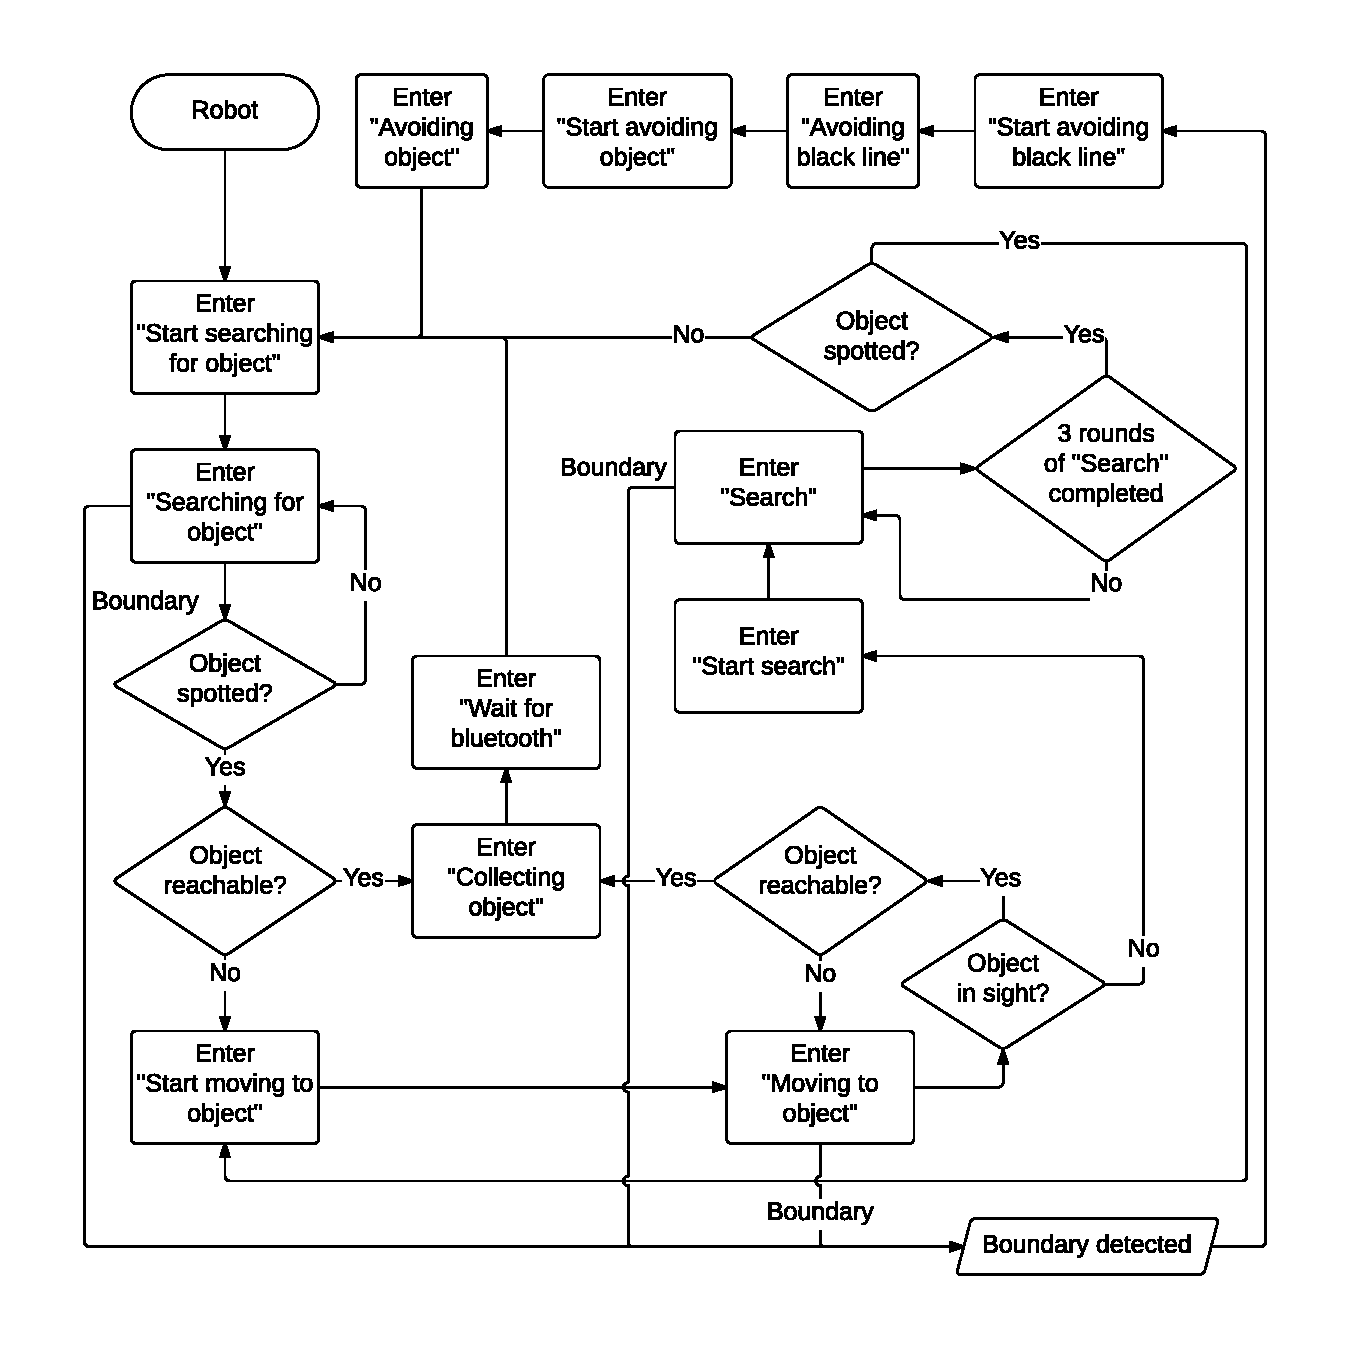
\includegraphics[width=\textwidth]
     {graphics/RobotBehaviour.pdf}}
     \caption{\label{fig:robot-behaviour} The robot's different states and their connections}
\end{figure}
